\todo[inline]{Problème des entrées, comment gérer SM ?}

L'analyse dynamique consiste à se baser sur une ou des exécutions particulières d'un programme pour inférer des propriétés sur son fonctionnement.
Elle demande donc de se munir d'une langage modélisant le fonctionnement de la machine durant l'exécution du programme, d'une sémantique concrète de l'assembleur utilisé et de lancer l'évaluation sémantique du programme sur une ou plusieurs entrées.
Les entrées d'un programme sont par exemple les paramètres passés lors de l'appel au programme, l'état de la machine lors du démarrage, les données lues depuis la mémoire et les saisies faites par l'utilisateur au clavier ou à la souris lors de l'exécution s'il s'agit d'une application dotée d'une interface graphique.

Nous définirons dans ce chapitre une sémantique simplifiée pour un langage assembleur permettant, à l'instar de \xq\ et \xs, l'auto-modification et le chevauchement de code. Nous expliquerons ensuite comment séparer une exécution d'un programme auto-modifiant en plusieurs sous-exécution non auto-modifiantes afin d'utiliser des techniques standard d'analyse sur chacune de ces sous-exécutions.

\section{Sémantique concrète pour un langage assembleur}

\paragraph{Représentation de la mémoire et des registres.}
On peut voir la mémoire comme un tableau contenant la pile et le tas, indexés sur les entiers. Les registres sont des variables distinctes de la mémoire et sont en nombre limité. Enfin, pour pouvoir gérer l'adressage indirect : \texttt{[eax]} fait référence à la valeur en mémoire à l'adresse contenue dans \eax, on ajoute les pointeurs vers une variable. Ces éléments sont définis formellement à la définition \ref{def:sem_conc_var}.

\begin{rem}
 Avec cette définition, une valeur en mémoire peut pointer vers un registre. De même un registre peut pointer vers un autre registre.
 Ces deux possibilités ne sont pas réalisables avec l'assembleur \xq\ ou \xs.
\end{rem}


\begin{defi}
On définit les symboles $x\in\BX$ comme constitués de variables $v\in\BV$ et de pointeurs $p\in\BP$ vers des variables. $\BV$ contient un ensemble fini de registres $a\in\BA$ et un tableau de taille finie $\BT=\textlbrackdbl 0,\ T\textrbrackdbl$. Les éléments de $\BP$ sont des pointeurs vers une variable : $\{[v],\ v\in \BV\}$.
Les valeurs possibles pour les variables sont dans $\BN$.
\label{def:sem_conc_var}
\end{defi}

\paragraph{Langage assembleur simplifié.} Nous allons définir un langage intermédiaire dans lequel on peut transcrire chaque instruction \xq\ en une liste d'instructions atomiques de notre langage simplifié.
Les instructions \xq\ sont disponibles à différentes adresses entières. 
Les instructions atomiques sont de plusieurs type explicités en définition \ref{def:sem_instructions} : le premier consiste en l'assignation.
Il est possible d'assigner un symbole ou une combinaison de symboles (à l'aide d'une fonction sur les entiers) à un symbole. 
Le second type d'instruction regroupe les sauts inconditionnels et conditionnels.
On distingue également l'instruction \texttt{end} forçant l'arrêt du programme.

\begin{defi}
Les instructions atomiques d'un programme sont de ce type, quelle que soit la fonction totale g de $\BN^m$ dans $\BN$ :\\
$inst:=\ $\emph{$x\leftarrow g(x_1, ..., x_m)$ $|$ goto $x$ $|$ if $x$ then $goto\ x'$ $|$ end}
\label{def:sem_instructions}
\end{defi}


% \paragraph{Exemples naïfs de la représentation d'instructions assembleur \xq.}
La figure \ref{fig:sem_exemples_insts} donne des exemples de transcription d'instructions \xq\ dans le langage défini précédemment. 
Ils sont naïfs au sens que les instructions \xq\ sont plus complexes et un simple \sub\ provoque des effets de bord modifiant des registres. Ce point sera développé par la suite lorsque nous discuterons des implémentations possibles pour cette sémantique concrète.
\\

\begin{figure}
 \begin{center}
  \begin{tabular}{|l|l|}
   \hline
   Instruction \xq & Instructions atomiques équivalentes\\
   \hline
   mov eax, 3 & $eax\leftarrow 3$ \\
   \hline
   mov [eax], 4 & $[eax]\leftarrow 4$ \\
   \hline
   mov [eax+1], 5 & $tmp\leftarrow addition(eax, 1)$ \\
    & $[tmp]\leftarrow 5$ \\
   \hline
   jmp eax & $goto\ eax$ \\
   \hline
   sub eax, 3 & $eax\leftarrow soustraction(eax, 3)$ \\
   \hline
  \end{tabular}
 \end{center}
\caption{Exemple de transcription d'instructions \xq\ dans le langage assembleur simplifié}
\label{fig:sem_exemples_insts}
\end{figure}


Comme nous avons vu dans les parties précédentes, un programme est simplement composé d'un ou plusieurs blocs d'octets à charger en mémoire. Une fois ces segments chargés dans le tableau $\BT$ représentant la mémoire, le point d'entrée du programme est placé dans le registre \texttt{ep}.


% \begin{defi}
% L'adresse 
% \label{def:sem_programme}
% \end{defi}

% 
%On note $\PMN$ l'ensemble des parties de $\BN$ de taille inférieure ou égale à M $\in\BN$ en excluant l'ensemble vide (représenté par $\bot$).

Pour faire le lien entre la machine et les instructions exécutées, il est nécessaire de pouvoir désassembler des instructions en mémoire. C'est le rôle de l'opérateur de désassemblage (définition \ref{def:sem_desassembleur}).

\begin{defi}
% On appelle $D$ l'opérateur de désassemblage qui à une adresse de la mémoire $\BT$ associe une instruction et la taille de cette instruction dans $\BN$. \\
On appelle $D$ l'opérateur de désassemblage qui à une adresse de la mémoire $\BT$ associe une liste d'instructions atomiques et la taille de cette instruction dans $\BN$. \\
Pour toute adresse $t\in\BT$, on note $D(t)=d_1..d_n$ et $D_S(t)$ respectivement la suite d'instructions atomiques à l'adresse $t$ et la taille de cette instruction.\\
Dans le cas où il n'y a pas d'instruction valide à l'adresse $t$, $D(t)=\bot$ et $D_S(t)=0$.
\label{def:sem_desassembleur}
\end{defi}

Une sémantique concrète cherche à définir les opérations de chaque instruction de la manière la plus précise qu'il soit afin de pouvoir simuler une exécution réelle du programme.
Pour cela on va utiliser une store qui conserve l'état des variables lors de l'exécution du programme.
Toute variable non initialisée a la valeur spéciale $\bot$ tandis que les variables définies ont des valeurs entières (définition \ref{sem_store_dynamique}).

\begin{defi}
 Un store dynamique associe à chaque variable une valeur : $\Theta:\BV\rightarrow\BN\cup\{\bot\}$.\\
 Si v est une variable et n une valeur, on note $\Theta[v\leftarrow n]$ l'assignation de v à n dans $\Theta$.
\label{sem_store_dynamique}
\end{defi}

Pour permettre l'adressage indirect on doit également définir le store sur l'ensemble des pointeurs.
La définition \ref{sem_store_dynamique_pointeurs} étend la notion de store aux pointeurs afin que chaque symbole ait une valeur.


\begin{defi}
 Définissons une extension $\Theta_X$ d'un store $\Theta : \BV\rightarrow\BN\cup\{\bot\}$ à $\BX\rightarrow\BN\cup\{\bot\}$. Soit $x\in\BX$.
 \begin{itemize}
  \item Si $x\in\BV$ : $\Theta_X(x)=\Theta(x)$
  \item Sinon, $x\in\BP$ : $x=\textlbrackdbl v\textrbrackdbl$ avec $v\in\BV$.
  \begin{itemize}
   \item Si $\Theta(v)=\bot$ alors $\Theta_X(x)=\bot$
   \item Si $\Theta(v)\in\BN$ et $\Theta(v)\notin\BT$ alors $\Theta_X(x)=\bot$
   \item Sinon $\Theta(v)\in\BN$ et $\Theta(v)\in\BT$, alors $\Theta_X(x)=\Theta(\Theta(v))$.
  \end{itemize}
 \end{itemize}
  De même on étend l'opération d'assignation d'une valeur à un symbole de la manière suivante. Soit $x\in\BX$ et $n\in\BN$.
  \begin{itemize}
  \item Si $x\in\BV$ : $\Theta_X[x\leftarrow n]$ est équivalent à $\Theta[x\leftarrow n]$.
  \item Sinon, $x\in\BP$ : $x=\textlbrackdbl v\textrbrackdbl$ avec $v\in\BV$.
    \begin{itemize}
   \item Si $\Theta(v)=\bot$ alors l'assignation n'a aucun effet
   \item Si $\Theta(v)\in\BN$ et $\Theta(v)>T$ alors l'assignation n'a aucun effet
   \item Sinon $\Theta(v)\in\BN$ et $\Theta(v)\in\BT$, alors $\Theta_X[x\leftarrow n]$ se résoud par $\Theta[\Theta(v)\leftarrow n]$.
  \end{itemize}
  \end{itemize}
\label{sem_store_dynamique_pointeurs}
\end{defi}

\paragraph{Règles de transition.}
Les états d'exécution sont de la forme \textlangle$t, \Theta_X$\textrangle\ où $t$ est une adresse ou l'adresse invalide (ou finale) $\bot$. À chaque instruction exécutée, il y a une transition \textlangle$t, \Theta_X$\textrangle$\rightarrow$\textlangle$t', \Theta_X'$\textrangle.\\
Si il y a une suite de transitions amenant d'un état \textlangle$t, \Theta_X$\textrangle\ à l'état \textlangle$t', \Theta_X'$\textrangle, on note \textlangle$t, \Theta$\textrangle$\rightarrow^*$\textlangle$t', \Theta_X'$\textrangle.\\
Un programme s'arrête en partant de l'état initial \textlangle$ep, \Theta_X$\textrangle\ où \texttt{ep} est son point d'entrée si et seulement si \textlangle$ep, \Theta_X$\textrangle$\rightarrow^*$\textlangle$\bot, \Theta_X'$\textrangle. Le programme dans ce cas s'arrête à la première occurrence d'une adresse invalide $\bot$.

On définit par la suite la sémantique des instructions atomiques et on étend donc les états d'exécution à celles-ci : on note \textlangle$t:d_1..d_n, \Theta_X$\textrangle\ l'état \textlangle$t, \Theta_X$\textrangle\ sur lequel il y a les instructions atomiques $d_1..d_n$ à évaluer.
À partir d'un état \textlangle$t, \Theta_X$\textrangle, on commence par déterminer les instructions atomiques à évaluer à l'aide de l'opérateur de désassemblage : on arrive à un état \textlangle$t:D(t), \Theta_X$\textrangle=\textlangle$t:d_1..d_n, \Theta_X$\textrangle\ dans lequel on va pouvoir évaluer les instructions atomiques l'une après l'autre. Une fois que toutes ces instructions ont été évaluées et si aucune d'elle n'a provoqué de saut vers une adresse différente, on passe à l'instruction qui suit séquentiellement à l'adresse $t+D_S(t$\textrangle.

L'état initial du store est : $\forall v\in\BV, \Theta_X(v)=\bot$ et l'on part du point d'entrée \texttt{ep}. Les règles de transition suivantes permettent d'aboutir à une adresse finale ou invalide $\bot$ si le programme termine.

% \begin{tabbing}
% \textlangle$t:x\leftarrow g(x_1, ..., x_m),\ \Theta_X$\textrangle\ \=$ \longrightarrow $ \textlangle$t+D_S(t),\ \Theta_X[x\leftarrow\bot]$\textrangle~~~~~~~~~~~~~~~~~~~~~~~~~~~~~~~\=si $\exists i, \Theta_X(b_i)=\bot$\\
%                                                                    \>$ \longrightarrow $ \textlangle$t+D_S(t),\ \Theta_X[x\leftarrow g(\Theta_X(b_1),...,\ \Theta_X(b_m))]$\textrangle \> sinon\\ \\
% 
% \textlangle$t:goto\ x,\ \Theta_X$\textrangle\>$\longrightarrow $ \textlangle$\Theta_X(x),\ \Theta_X$\textrangle\> \\ \\
% 
%  \textlangle$t:if\ x\ then\ goto\ x',\ \Theta_X$\textrangle\>$ \longrightarrow $ \textlangle$\Theta_X(x'),\ \Theta_X$\textrangle\ \>si $\Theta_X(x)=1$\\
% 									    \>$ \longrightarrow $ \textlangle$ t+D_S(t),\ \Theta_X$\textrangle\ \>sinon\\ \\
% 
% \textlangle$t\notin\BT,\ \Theta_X$\textrangle\>$ \longrightarrow $ \textlangle$\bot,\ \Theta_X$\textrangle\\
% \textlangle$t:end,\ \Theta_X$\textrangle\>$ \longrightarrow $ \textlangle$\bot,\ \Theta_X$\textrangle
% \end{tabbing}


\begin{center}
\begin{tabular}{lcl}
% \hline
\textlangle$t\in\BT;\ \Theta_X$\textrangle & $\longrightarrow$ & \textlangle$t:D(t);\ \Theta_X$\textrangle  \\
& & \\
% \hline
\textlangle$t:x\leftarrow g(x_1, ..., x_m), d_2..d_n;\ \Theta_X$\textrangle & $\longrightarrow$  & \textlangle$t:d_2..d_n;\ \Theta_X[x\leftarrow\bot]$\textrangle\  \\
 &   & ~~~si $\exists i, \Theta_X(b_i)=\bot$  \\
 & $\longrightarrow$  & \textlangle$t:d_2..d_n;\ \Theta_X[x\leftarrow g(\Theta_X(b_1),...,\ \Theta_X(b_m))]$\textrangle\    \\
  &   & ~~~sinon  \\
% \hline
& & \\
\textlangle$t:goto\ x, d_2..d_n;\ \Theta_X$\textrangle & $\longrightarrow$ & \textlangle$\Theta_X(x);\ \Theta_X$\textrangle  \\
% \hline
& & \\
\textlangle$t:if\ x\ then\ goto\ x',\ \Theta_X$\textrangle\ & $\longrightarrow$ & \textlangle$\Theta_X(x'),\ \Theta_X$\textrangle\\\
  &   & ~~~si $\Theta_X(x)=1$  \\
 & $\longrightarrow$ & \textlangle$ t+D_S(t),\ \Theta_X$\textrangle\\
   &   & ~~~sinon  \\
% \hline
& & \\
\textlangle$t:end, d_2..d_n;\ \Theta_X$\textrangle\ & $\longrightarrow$ & \textlangle$\bot;\ \Theta_X$\textrangle  \\
% \hline
& & \\
\textlangle$t:\bot;\ \Theta_X$\textrangle\ & $\longrightarrow$ & \textlangle$\bot;\ \Theta_X$\textrangle  \\
% \hline
& & \\
\textlangle$t\in\BT:\emptyset;\ \Theta_X$\textrangle & $\longrightarrow$ & \textlangle$t+D_S(t);\ \Theta_X$\textrangle  \\
& & \\
\textlangle$t\notin\BT;\ \Theta_X$\textrangle\ & $\longrightarrow$ & \textlangle$\bot;\ \Theta_X$\textrangle  \\
% \hline
\end{tabular}
\end{center}

Dans la suite de ce chapitre nous appelons évaluation sémantique ou \texttt{sem\_eval} la fonction qui, à une adresse $t$ et un store $\Theta_X$, associe l'état sur les instructions \xq\ suivant : si $t'$ et $\Theta_X'$ sont les premières valeurs vérifiant \textlangle$t, \Theta$\textrangle$\rightarrow^*$\textlangle$t', \Theta_X'$\textrangle\ alors \texttt{sem\_eval}$(t, \Theta_X)=(t', \Theta_X')$.


\subsection{Assembleur et langage intermédiaire}
En pratique pour analyser un programme assembleur on veut en avoir un représentation dont on connaît la sémantique concrète.
On va pour cela réécrire le programme dans un langage intermédiaire et effectuer les analyses sur le programme en langage intermédiaire.

Une des difficultés rencontrées dans la transformation d'un langage assembleur en langage intermédiaire est la richesse sémantique du langage \xq\ qui contient des centaines d'instructions et utilise de nombreux registres et drapeaux du processeur.
L'instruction \texttt{sub eax, b} par exemple soustrait l'opérande \texttt{b} à \eax\  en stockant le résultat de l'opérant dans \eax.
Le mnémonique \texttt{sub} désigne une vingtaine de variantes de la soustraction selon la taille des opérandes pris en compte. Elle effectue l'opération \texttt{eax-b} et met à jour les drapeaux CF et OF indiquant un dépassement de valeur entière, le drapeau de signe SF, le drapeau ZF (à 1 si le résultat est nul) et celui de parité PF.

Une instruction assembleur va donc être traduite en une ou plusieurs instructions atomiques dans le langage intermédiaire que l'on sait équivalentes sémantiquement à l'instruction \xq\ et dont on a une sémantique concrète pour les exécuter.
Une difficulté pratique vient de la richesse du langage \xq\ : écrire l'équivalence de chacun de ses instructions dans le langage intermédiaire choisi est une tâche longue et prône aux erreurs, notamment lors de l'analyse de la documentation. Pour cette raison nous avons rapidement choisi de nous orienter vers des langages intermédiaire pour lesquels cette étape a déjà été réalisée.

\subsection{Revue de littérature et implémentations}
\todo[inline]{BAP: \\
Jakstab: \\
TraceSurfer: \\
Renovo : \\
LLVM : \\
Implem en C: \\
TraceSurfer: \\
Pin : \\
Xed : \\
}

\section{Auto-modification et vagues}
Si on reprend l'exemple de code auto-modifiant de la figure \ref{fig:unevague_v0}, on peut construire trois représentations en mémoire des parties exécutables du programme.
La première correspond à la vision du programme lors de son chargement : la section .text est dans son état initial.
La seconde est celle après que la première modification du programme faite à l'adresse \adr{8048086} et la troisième après la seconde modification faite à l'adresse \adr{804808b}.
En fait vu qu'aucune des adresses modifiées par la première instruction auto-modifiante n'est exécutées avant que la seconde modification ne soit faite, on peut regrouper les deux instructions auto-modifiantes et considérer que le programme n'a que deux représentations en mémoire : la représentation initiale et la représentation au moment où l'instruction modifiée à l'adresse \adr{8048091} est exécutée.

Dans ce découpage informel on appelle vague une représentation mémoire à un instant donné. 
L'exécution d'un programme est alors caractérisé par une suite d'exécutions sur des vagues successives comme représenté en figure \ref{fig:vagues_visuel}. Les instructions qui sont présentes dans la trace sont colorées en rose tandis que le point d'entrée et la dernière instruction sont en orange et bleu clair, respectivement.
On passe d'une vague $k$ à la vague suivante $k+1$ lorsqu'une adresse mémoire écrite dans la vague $k$ est exécutée.
Ainsi dans une vague $k$, toutes les instructions exécutées ont été écrites au moins à la vague $k-1$. 
En ce sens chacune des vagues, prise indépendamment des autres, ne présente pas d'auto-modification.

Nous détaillerons par la suite ce qu'est une trace d'exécution pour l'analyse dynamique ainsi que la sémantique d'enchaînement des vagues.

\begin{figure}
 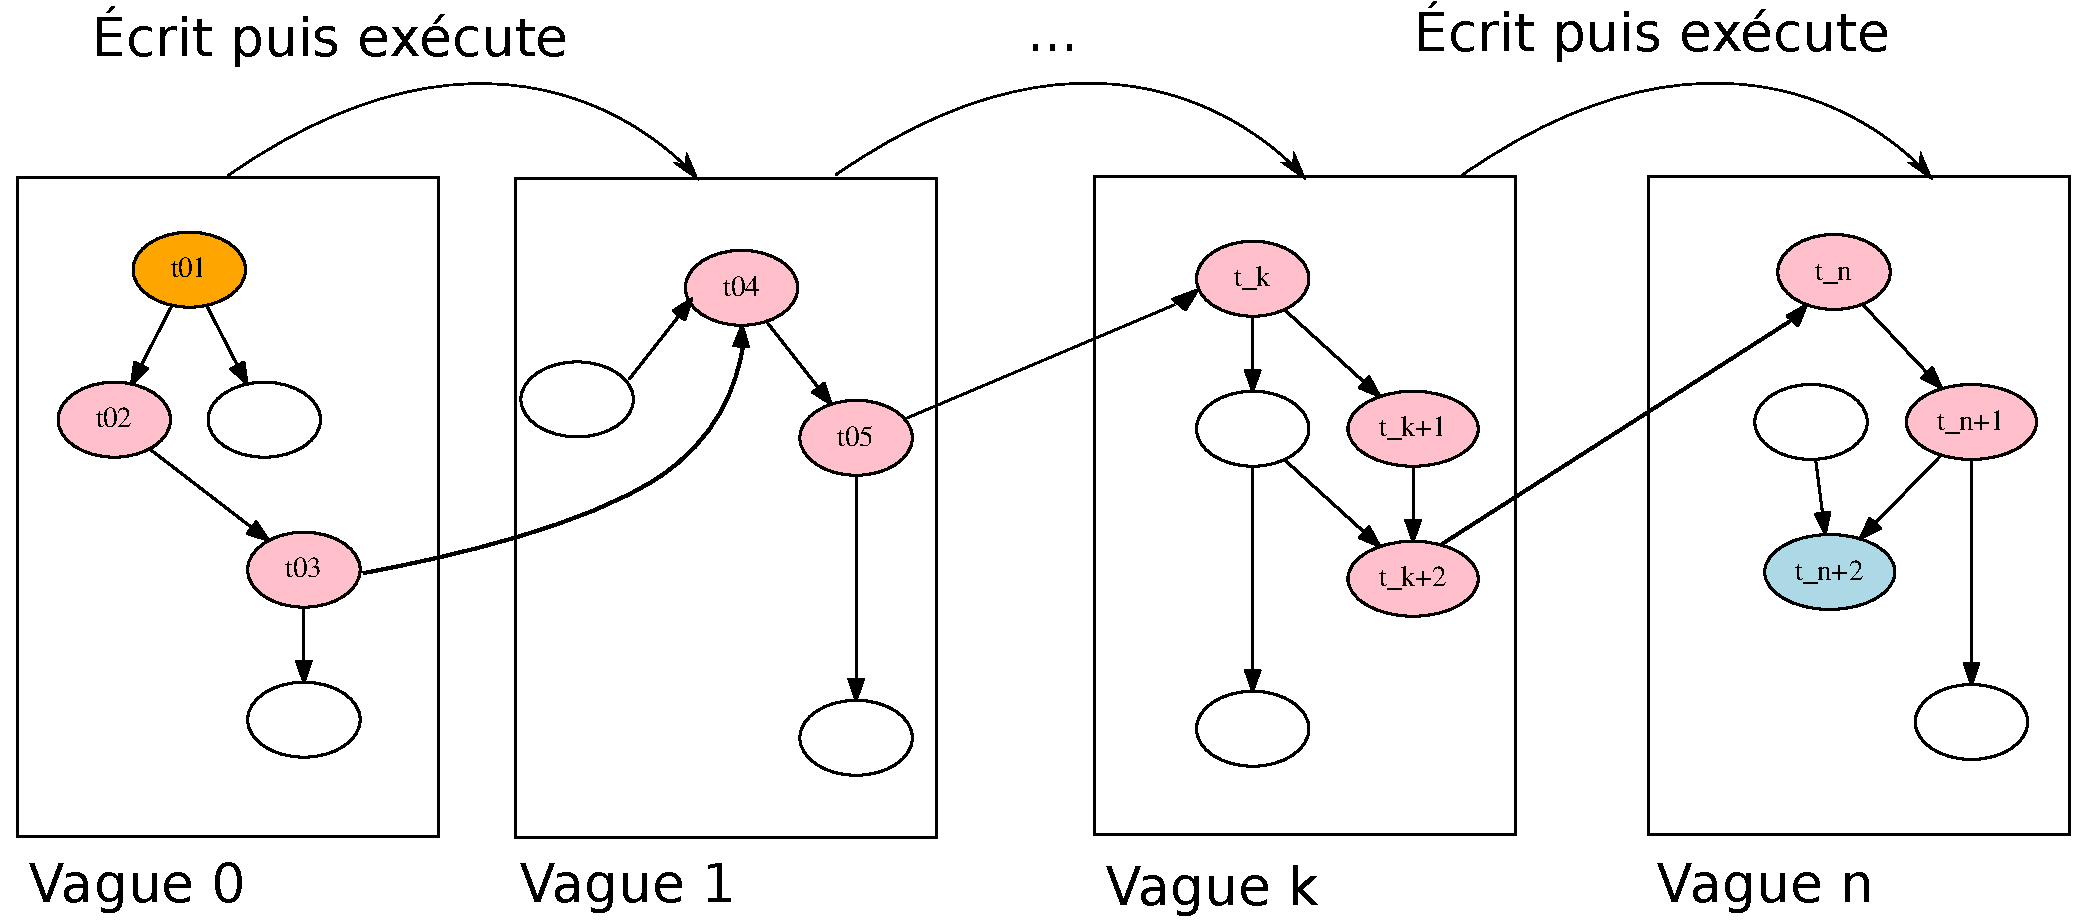
\includegraphics[width=1.0\textwidth]{supports/automodification/phases2_final.pdf}
 \caption{Vision informelle des vagues}
 \label{fig:vagues_visuel}
\end{figure}


\subsection{Revue de littérature}
La notion de vague présentée dans ce chapitre a été développée dans les thèse de Calvet \cite{Calvet2013} et Reynaud \cite{Reynaud2010}.
Elle est similaire à la notion de \emph{phase} présentée par Debray et Patel \cite{DP10} et utilisée pour automatiser la suppression de la protection d'un binaire.
En général la suppression des protections se fait à l'aide d'une analyse dynamique et d'une image de la mémoire à un instant donné au cours de l'exécution. C'est cette image mémoire qui sera considéré comme était le programme d'origine. La difficulté réside alors dans le choix de l'instant où prendre l'image mémoire.


\subsection{Trace, niveaux d'exécution et vagues}
Le programme exécuté a pour sources principales de données les registres et la mémoire constituée de la pile et du tas qui sont tous les deux adressables par des entiers. Une variable d'un programme est donc soit un registre du processeur soit une adresse mémoire, comme indiqué en définition \ref{def:variable}.
\begin{defi}
On définit l'ensemble $\BV$ des variables comme contenant un ensemble fini de registres $a\in\BA$ et un tableau de taille finie $\mathbb{T}=\textlbrackdbl 0,\ t\textrbrackdbl$.
\label{def:variable}
\end{defi}

En utilisant la sémantique concrète précédemment définie on est capable, à partir d'un ensemble de valeurs initiales pour les registres et la mémoire, d'exécuter un programme sur cette entrée.
Une trace d'exécution d'un programme est simplement l'enchaînement des instructions auxquelles l'exécution du programme a fait appel. Si on note $I_i$ une instruction dynamique, la trace d'exécution est $T=I_1, I_2, ..., I_n$ où $I_n$ est la dernière instruction du programme.

Nous définissons une instruction dynamique (définition \ref{def:ensembles_inst_dyn}) par son adresse, les adresses mémoires sur lesquelles elle est codée et l'instruction machine correspondant. Ces informations sont données par un désassemblage atomique d'une instruction à l'adresse mémoire spécifiée.
Afin de pouvoir séparer la trace d'exécution selon le moment où chaque instruction a été écrite, nous définissons aussi pour chaque instruction l'ensemble des variables sur lesquelles elle provoque une écriture. Cette information est donnée par la sémantique concrète choisie.

\begin{defi}
On note $D$ une instruction dynamique constituée des éléments suivants.
\begin{itemize}
 \item \da{D} l'adresse mémoire de l'instruction dynamique
 \item \dc{D} le segment des adresses mémoire sur lequel \di{D} est codée
 \item \di{D} l'instruction machine à l'adresse \da{D}
%  \item \dr{D_i} l'ensemble des variables sur lesquelles l'exécution de \di{D_i} provoque une lecture
 \item \dw{D} l'ensemble des variables sur lesquelles l'exécution de \di{D} provoque une écriture
\end{itemize}
\label{def:ensembles_inst_dyn}
\end{defi}

Nous avons donc, pour une trace d'exécution donnée, des vagues successives $1, 2, ..., n$.
Au cours de l'exécution du programme on définit, pour chaque adresse en mémoire $m$, un niveau d'écriture $W^M[m]$.
correspondant à la dernière vague $k$ durant laquelle une instruction a modifié la valeur à l'adresse $m$.


Une instruction $D$ a un niveau d'exécution $X$, comme indiqué en définition \ref{def:write_exec_levels}.
Elle a également a un niveau d'écriture $W_D$ qui est le niveau d'écriture le plus élevé parmi les adresses sur lesquelles elle est codée : $W_D=max(W^M[a],\ a\in\ $\dc{D_i}$)$.


\begin{defi}
Nous définissons une trace d'exécution comme la donnée d'une suite $T=t_1, t_2, ..., t_n$ composée de triplets de la forme $t_i=(i, D_i, X_i)$ tels que
\begin{itemize}
 \item $D_i$ est la $i^{eme}$ instruction exécutée.
 \item Avant l'exécution de l'instruction $D_i$, le niveau d'exécution est \texttt{$X_{i-1}$}.
 \item Après l'exécution de l'instruction $D_i$, le niveau d'exécution est \texttt{$X_i$}.
\end{itemize}
\label{def:write_exec_levels}
\end{defi}

\begin{propri}
 Si le niveau d'exécution courant est $X$, le niveau d'exécution de l'instruction à exécuter $D_i$ est :\\
 $X=max(X, W_D+1)$ avec $W_D=max(W^M[a],\ a\in\ $\dc{D_i}$)$.\\
 Après l'exécution de $D_i$, les niveaux d'écriture dans la mémoire sont mis à jour de la manière suivante :\\
 $\forall a\in$ \dw{D_i}, $W^M[a]=X$.
\label{propri:niveau_exec}
\end{propri}

En pratique une instruction $D$ écrite par une instruction ayant pour niveau d'exécution $k$ puis directement exécutée aura pour niveau d'écriture $W_D=k$ et pour niveau d'exécution $X=k+1$. Ce comportement est formalisé par la propriété \ref{propri:niveau_exec}.

On définit alors formellement la vague $k$ selon la définition \ref{def:vagues} et l'algorithme \ref{algo:analyse_dyn_vagues} permet d'exécuter un programme dynamiquement avec la sémantique concrète choisie tout en déterminant les niveaux d'exécution de d'écriture au fur et à mesure de l'exécution. La sortie de l'algorithme \ref{algo:analyse_dyn_vagues} est la trace d'exécution et la liste des vagues reconstruites.
\\

Reprenons l'exemple du programme auto-modifiant de la figure \ref{fig:unevague_trace}.
La figure \ref{fig:unevague_trace} donne une trace d'exécution de ce programme en détaillant les informations sur chaque instruction dynamique ainsi que les niveaux d'écriture et d'exécution de chaque instruction.
Au départ toute la mémoire est dans son état d'origine et a pour niveau d'exécution 0. Lorsque l'instruction $D_0$ est exécutée, il n'y a pas eu d'auto-modification donc le niveau d'écriture est 0 et le niveau d'exécution est 1.
Les instructions $D_3$ et $D_4$ provoquent une auto-modification : les octets aux adresses \adr{0x8048091} et \adr{0x8048092} sont modifiés et leurs niveaux d'écriture deviennent donc le niveau d'exécution courant, soit 1.
Lorsque l'exécution atteint $D_5$, qui a été modifié, le niveau d'écriture est 1 donc le niveau d'exécution devient 2.
L'instruction suivante $D_6$ fixe la valeur de \edi\ à 2 puis les instructions suivantes provoquent l'affichage de \edi.

Cette trace d'exécution est donc composée de deux vagues : la vague initiale, $v_0$ composée de l'état de la mémoire avant l'exécution de la première instruction et la vague $v_1$ contenant l'état de la mémoire juste après l'exécution de $D_4$ et avant l'exécution de la première instruction modifiée $D_5$.




\begin{defi}
 Étant donné une trace d'exécution $T=t_1, ..., t_n$ avec $t_i=(i, D_i, X_i)$ et $k\in\{X_j, 1\leq i\leq n\}$, on appelle vague $k$ l'état de la mémoire juste après l'exécution de la dernière instruction ayant pour niveau d'exécution $k$.
 C'est à dire l'état de la mémoire juste après l'instruction $D_j$ avec $X_{j+1}>k$.
 \label{def:vagues}
\end{defi}

% \begin{algorithm}[H] %or another one check
% \caption{Mise à jour des niveaux d'exécution et d'écriture lors de l'exécution d'une instruction}
% \SetAlgoLined
% \KwIn{La mémoire, l'opérateur de niveau d'écriture, une instruction dynamique et le niveau d'exécution courant}
% \KwResult{L'opérateur de niveau d'écriture et le niveau d'exécution courant mis à jour}
% \SetKwProg{Fn}{}{}{}
% \SetKwFunction{FRecurs}{calculNiveau}
% \Fn(
% ){\FRecurs{M, $W^M$, D, X}}{
% $W_D \leftarrow\ max(W^M[a],\ a\in\ $\dc{D}$)$\\
% $X \leftarrow\ max(X,\ W_D+1)$ \\
% \For {$m\in\ $\dw{D}}{
%   $W^M[m]\leftarrow\ X$
% }
% \Return ($W^M$, X)
% }
% \label{algo:update_vagues}
% \end{algorithm}

\begin{algorithm}[H] %or another one check
\caption{Mise à jour du niveau d'exécution d'une instruction}
\SetAlgoLined
\KwIn{La mémoire, l'opérateur de niveau d'écriture, une instruction dynamique et le niveau d'exécution courant}
\KwResult{Le niveau d'exécution courant mis à jour}
\SetKwProg{Fn}{}{}{}
\SetKwFunction{FRecurs}{MAJExecution}
\Fn(
){\FRecurs{M, $W^M$, D, X}}{
$W_D \leftarrow\ max(W^M[a],\ a\in\ $\dc{D}$)$\\
$X \leftarrow\ max(X,\ W_D+1)$ \\
\Return X
}
\label{algo:update_exec_level}
\end{algorithm}

\begin{algorithm}[H] %or another one check
\caption{Mise à jour des niveaux d'écriture lors de l'exécution d'une instruction}
\SetAlgoLined
\KwIn{La mémoire, l'opérateur de niveau d'écriture, une instruction dynamique et le niveau d'exécution courant}
\KwResult{L'opérateur de niveau d'écriture mis à jour}
\SetKwProg{Fn}{}{}{}
\SetKwFunction{FRecurs}{MAJEcriture}
\Fn(
){\FRecurs{M, $W^M$, D, X}}{
\For {$m\in\ $\dw{D}}{
  $W^M[m]\leftarrow\ X$
}
\Return $W^M$
}
\label{algo:update_write_level}
\end{algorithm}

\begin{figure}
\begin{center}
\begin{tabular}[b]{|l|l|l|l|l|l|l|}
\hline
i & \da{D_i} & \dc{D_i} & \di{D_i} & \dw{D_i} & $W_i$ & $X_i$ \\
\hline
& 8048060  &  (...)         	        & Pile -> RWX &  & 0 & 1 \\ 
1 & 804807c  &  [804807c, 8048080]         &  mov    edi, 0x0 & edi & 0 & 1 \\
2 & 8048081  &  [8048081, 8048086]         &  mov    eax, 0x8048091 & eax & 0 & 1 \\
3 & 8048086  &  [8048086, 804808a]         &  mov    [eax], 0xeb & 0x8048091 & 0 & 1 \\
4 & 804808b  &  [804808b, 8048090]         &  mov    [eax+1], 0x7 & 0x8048092 & 0 & 1 \\
5 & 8048091  &  [8048091, 8048092]         &  jmp    80480a1 <edi3> &  & 1 & 2  \\
6 & 804809a  &  [804809a, 804809d]         &  mov    edi,0x2 & edi & 0 & 2\\
7 & 804809f  &  [804809f, 80480a0]         &  jmp    80480a8 <fin> &  & 0 & 2\\
 & 80480a8  &  (...)		        &  Affiche edi &  & 0 & 2\\
 & 80480c3  &  (...)		        &  Quitte &  & 0 & 2\\
\hline
\end{tabular}
\end{center}
\caption{Trace d'exécution du programme auto-modifiant de la figure \ref{fig:unevague_v0}}
\label{fig:unevague_trace}
\end{figure}

\begin{algorithm}[H] %or another one check
\caption{Analyse dynamique avec calcul des vagues}
\SetAlgoLined
\KwIn{Les registres R et une mémoire M dans laquelle un programme a été chargé à son point d'entrée \texttt{ep}}
\KwResult{La trace des instructions dynamiques chacune associée à leur niveau d'exécution et les différentes vagues de la trace}
\SetKwProg{Fn}{}{}{}
\SetKwFunction{FRecurs}{analyseDynamique}
\Fn(
% \tcc*[h]{C : matrice des associations possibles, i : numéro du prochain sommet de P à associer, F : liste des couples d'associations déjà faites}
){\FRecurs{R, M, ep}}{
\For{$m\in M$}{
  $W^M[m]\leftarrow 0$\\
}
$X\leftarrow 1$\\
$X_{-1}\leftarrow 0$\\
$i\leftarrow 0$\\
$T\leftarrow \emptyset$\\
$vagues\leftarrow \emptyset$\\
$eip\leftarrow ep$\\
\While {la fin du programme n'est pas atteinte} {
$i\leftarrow i+1$\\
~\\
$D\leftarrow decode(eip, M)$\\
$X\leftarrow MAJExecution(M, W^M, D, X)$\\
\If {$X \ne X_{-1}$}{
  $vagues\leftarrow vagues\cup \{(X_{-1}, M)\}$
}
$X_{-1} \leftarrow X$\\
~\\
$(eip, R, M)\leftarrow sem\_eval(eip, R, M)$\\
$W^M\leftarrow MAJEcriture(M, W^M, D, X)$\\
$T\leftarrow T\cup\{(i, D_i, X)\}$\\
}
\Return T, vagues
}
\label{algo:analyse_dyn_vagues}
\end{algorithm}

\begin{rem}
 Étant donné la définition croissante des vagues, la même instruction $D$ peut-être exécutée non seulement plusieurs fois dans la même vague mais également être présente à des vagues différentes.
\end{rem}

